% \bibliography{../src/bibliography}

In this chapter I give the background.

\section{Syntax}
\begin{itemize}
  \item Some generic stuff on syntax, hierarchical structure in language, and constituency in natural language referencing \citet{Carnie2010:constituent,Everaert+2015:structures}.
  \item Introduce the concept of \textit{acceptability judgements}, with the final chapter on syntactic evaluation in mind.
\end{itemize}

\section{Parsing}
\begin{itemize}
  \item Treebanks, in particular the Penn Treebank. Treebank preprocessing. CFGs, CNF, spans. Reference figure \ref{fig:trees}.
  \item The two conceptions of a tree: as a set of \textit{labeled spans} or as a set of \textit{anchored rules}.
  \item A labeled span is a triple $(\ell, i, j)$ of a syntactic label $\ell$ together the left and right endpoints $i$, $j$ that the label spans.
  \item An \textit{anchored rule} is a triple $(r, i, j)$ or four-tuple $(r, i, k, j)$, containing a CNF rule $r$ with span endpoints $i$, $j$, and a split-point $k$ of the left and right child $r$ is not a lexical rule.
  \item For the difference, consider the following two representations of the tree in figure \ref{fig:tree-cnf-spans} given in table \ref{tab:spans-rules}.
  \item Algorithms for parsing: global chart based, local transition based
  \item Dynamic programming inference versus search heuristics.
  \item Modelling types: generative, discriminative, log-linear, count-based, feature-based, neural network features.
\end{itemize}

% \begin{figure}
% 	\centering
%   \begin{subfigure}{0.72\textwidth}
% 		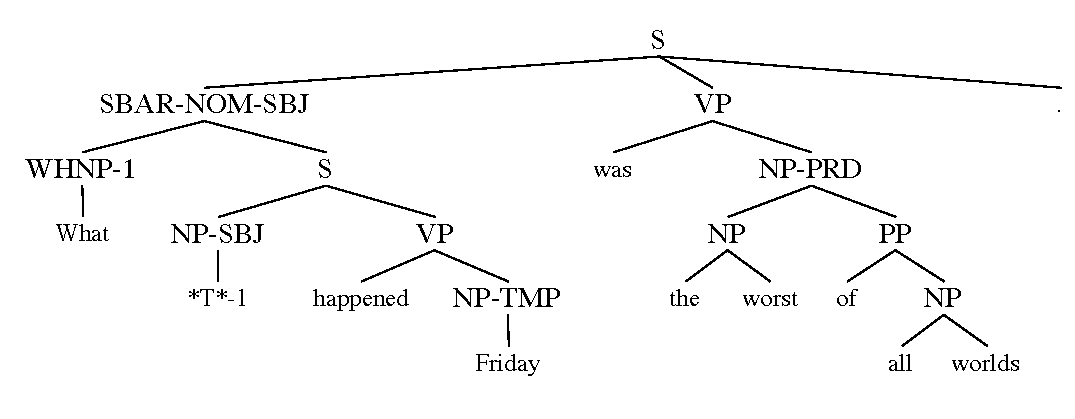
\includegraphics[width=\textwidth]{trees/original.pdf}
%     \caption{Original Penn Treebank tree.}
% 		\label{fig:tree-original}
% 	\end{subfigure}
% 	\begin{subfigure}{0.62\textwidth}
% 		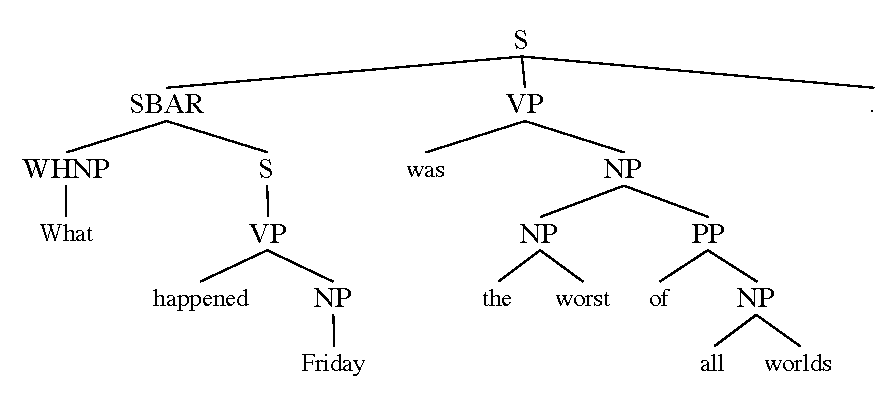
\includegraphics[width=\textwidth]{trees/simplified.pdf}
%     \caption{Function tags and traces removed.}
% 		\label{fig:tree-simplified}
% 	\end{subfigure}
% 	\begin{subfigure}{0.62\textwidth}
% 		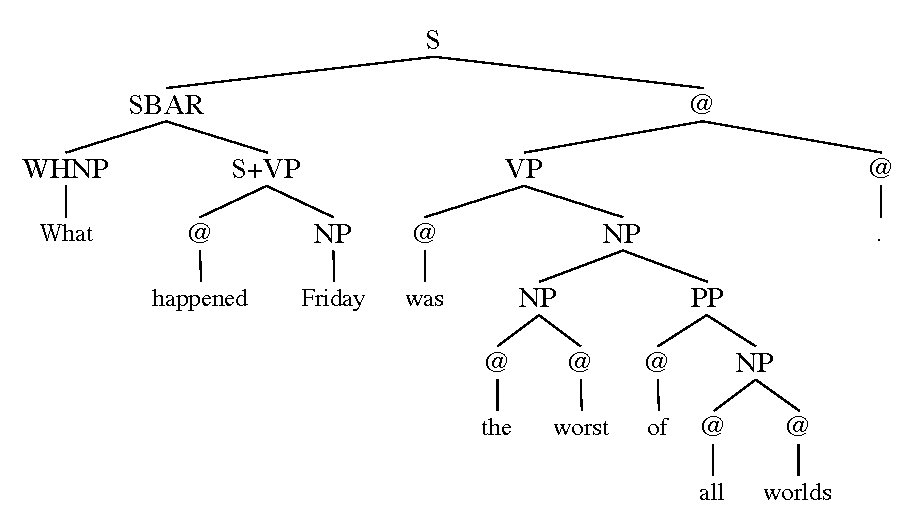
\includegraphics[width=\textwidth]{trees/binary.pdf}
%     \caption{Converted to normal form.}
% 		\label{fig:tree-cnf}
% 	\end{subfigure}
% 	\begin{subfigure}{0.9\textwidth}
% 		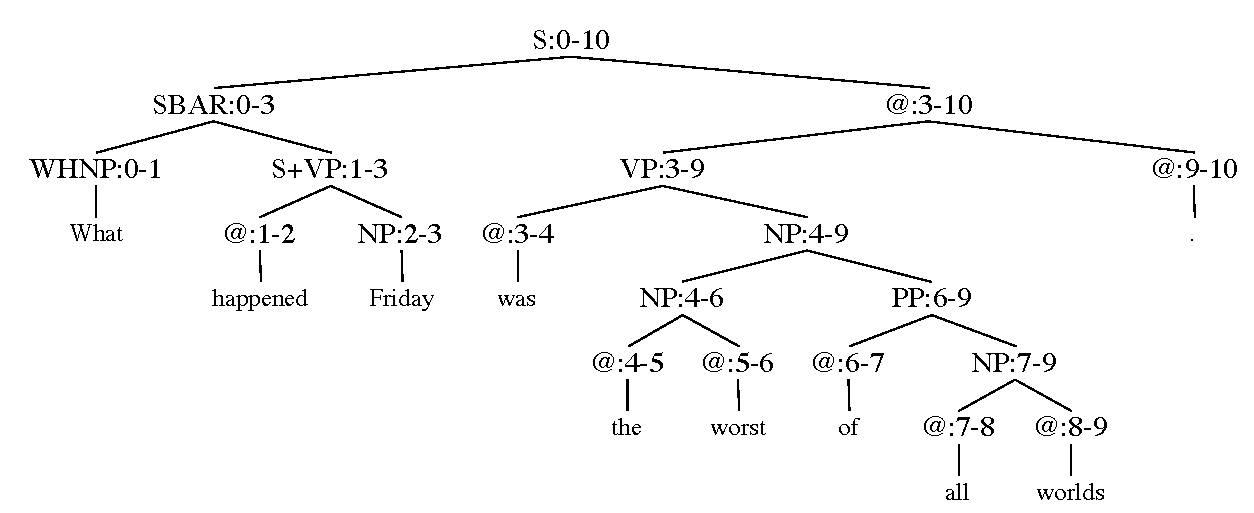
\includegraphics[width=\textwidth]{trees/spans.pdf}
%     \caption{In normal form with spans.}
% 		\label{fig:tree-cnf-spans}
% 	\end{subfigure}
%   \caption{Converting a treebank tree (withouth part-of-speech tags).}
%   \label{fig:trees}
% \end{figure}

\begin{figure}

  \begin{subfigure}[b]{\textwidth}
    \center
    \begin{tikzpicture}[scale=.6]
      \Tree [.S
        [.SBAR-NOM-SBJ
          [.WHNP-1 What ]
          [.S [.NP-SBJ *T*-1 ] [.VP happened [.NP-TMP Friday ] ] ] ]
        [.VP
          was
          [.NP-PRD [.NP the worst ] [.PP of [.NP all worlds ] ] ] ]
        . ]

    \end{tikzpicture}
    \subcaption{Original Penn Treebank tree.}
		\label{fig:tree-original}
  \end{subfigure}

  \begin{subfigure}[b]{\textwidth}
    \center
    \begin{tikzpicture}[scale=.6]
		  \Tree [.S
        [.SBAR [.WHNP What ] [.S [.VP happened [.NP Friday ] ] ] ]
        [.VP
          was
          [.NP [.NP the worst ] [.PP of [.NP all worlds ] ] ] ]
        $.$ ]

    \end{tikzpicture}
    \tiny
    \subcaption{Function tags and traces removed.}
		\label{fig:tree-simplified}
  \end{subfigure}

  \begin{subfigure}[b]{\textwidth}
    \center
    \begin{tikzpicture}[scale=.6]
		  \Tree [.S
        [.SBAR [.WHNP What ] [.S+VP [.$\varnothing$ happened ] [.NP Friday ] ] ]
        [.$\varnothing$
          [.VP
            [.$\varnothing$ was ]
            [.NP
              [.NP [.$\varnothing$ the ] [.$\varnothing$ worst ] ]
              [.PP [.$\varnothing$ of ] [.NP [.$\varnothing$ all ] [.$\varnothing$ worlds ] ] ] ] ]
          [.$\varnothing$ . ] ] ]

    \end{tikzpicture}
    \tiny
    \subcaption{Converted to normal form.}
		\label{fig:tree-cnf}
  \end{subfigure}

  \begin{subfigure}[b]{\textwidth}
    \center
    \begin{tikzpicture}[scale=.6]
		  \Tree [.S:0-10
        [.SBAR:0-3
          [.WHNP:0-1 What ]
          [.S+VP:1-3 [.@:1-2 happened ] [.NP:2-3 Friday ] ] ]
        [.@:3-10
          [.VP:3-9
            [.@:3-4 was ]
            [.NP:4-9
              [.NP:4-6 [.@:4-5 the ] [.@:5-6 worst ] ]
              [.PP:6-9
                [.@:6-7 of ]
                [.NP:7-9 [.@:7-8 all ] [.@:8-9 worlds ] ] ] ] ]
          [.@:9-10 . ] ] ]

    \end{tikzpicture}
    \tiny
    \subcaption{In normal form with spans.}
		\label{fig:tree-cnf-spans}
  \end{subfigure}

\caption{Converting a treebank tree (withouth part-of-speech tags).}
\label{fig:trees}
\end{figure}


\begin{table}[]
  \center
  \small
  \bgroup  % increase vertical space
  \def\arraystretch{1.5}  % increase vertical space
  \begin{tabular}{l|l}
    Labeled spans & Anchored rules \\
    \hline
    (S, 0, 10)     & (S $\to$ SBAR $\varnothing$, 0, 3, 10)  \\
    (SBAR, 0, 3)   & (SBAR $\to$ WHNP S+VP, 0, 1, 3)  \\
    (VP, 1, 3)     & (S+VP $\to$ $\varnothing$ NP, 1, 2, 3)  \\
    $\qquad\vdots$ & $\qquad\vdots$  \\
    (NP, 7, 9)     & (NP $\to$ $\varnothing$ $\varnothing$, 7, 8, 9)  \\
  \end{tabular}
  \caption{Two conceptions of the tree in \ref{fig:tree-cnf-spans}.}
  \label{tab:spans-rules}
  \egroup  % increase vertical space
\end{table}


\section{Language models}
\begin{itemize}
  \item Briefly mention some typical approaches for langugage modelling: count based n-gram with smoothing \citep{chen1999empirical,kneser1995improved}, neural n-gram \citep{bengio2003neural} and recurrent neural network \citep{mikolov2010recurrent}. Also mention some (early) syntactic approaches: count-based \citep{chelba2000structured,pauls2012treelets}, neural \citep{emami2005neural}, and top-down parsing related \citep{Roark2001}.
  \item Explain the metric perplexity.
  \item Briefly mentions some typical datasets and some benchmarks (dataset, perplexity, number of parameters, training time).
  \item Mention some downsides of the perplexity metric: conflating different sources of succes in next-word prediction (simple collocations, semantics, syntax).
  \item Note that there exists some alternatives to perplexity: adversarial evaluation \citep{Smith2012:adversarial}, subject-verb agreement \citep{Linzen+2016:LSTM-syntax} and grammatical acceptability judgments \citep{Linzen+2018:targeted}.
\end{itemize}


\section{Neural networks}
Introduce all the neural networks: \ff, \rnn, \lstm, etc.
\begin{itemize}
  \item We consider the neural networks as abstractions denoting certain parametrized functions.
  \item Let $\x$ and $\y$ be vectors in respectively $\reals^{n}$ and $\reals^{m}$.

  A \textit{feedforward neural network} is a parametrized function $\ff: \reals^{n} \to \reals^{m}$.

  A \textit{recurrent neural network} is a parametrized function \rnn that takes a sequence of vectors $(\x_i)_{i=1}^n = ( \x_1, \x_2, \dots, \x_n )$ in $\reals^{n}$ and produces a sequence of output vectors in $(\y_1,\y_2, \dots,\y_n )$ in $\reals^{m}$:
  \begin{align*}
    \rnn( (\x_i)_{i=1}^n ) &= ( \y_1, \y_2, \dots, \y_n ).
  \end{align*}
  Internally, the \rnn recursively applies an internal function $f: \reals^{n} \times \reals^{m} \to \reals^{m}$, also called the recurrent \textit{cell}, to the combined input of the current input and the output ouput of the previous timestep  with the input at that timestep, like
  \begin{align*}
    \y_{t} &= f(\x_t, \y_{t-1})  \\
      &= f(\x_t, f(\x_{t-1}, \y_{t-2}))  \\
      &\vdots \\
      &= f(\x_t, f(\x_{t-1}, f(\dots f(\x_{1}, \y_{0})))),
  \end{align*}
  where $\y_{0}$ is an initial vector that is does not depend on input.

  And \rnn can be applied to the inverse input sequence
  \begin{equation}
    \rev( (\x_i)_{i=1}^n ) \triangleq ( \x_n, \x_{n-1}, \dots, \x_1 ),
  \end{equation}
  that is, in \textit{backward} direction:
  \begin{align*}
    \rnn^B( (\x_i)_{i=1}^n )
      &= \rev( \rnn( \rev( (\x_i)_{i=1}^n ) ) ) \\
      &= \rev( \rnn( \x_n, \x_{n-1}, \dots, \x_1 ) \\
      &= \rev( \y_n, \y_{n-1}, \dots, \y_1 ) \\
      &= (\y_1,\y_2, \dots, \y_n ). \\
  \end{align*}
  For consistency we will refer to the \rnn in the regular, \textit{forward}, direction as $\rnn^F$. To stress the difference between the different outputs obtained from the two directions, we will denote the output vectors obtained in the regular, forward, direction with $\fw_i$ and the vectors obtained in the backward direction with $\bw_i$:
  \begin{align*}
    \rnn^B( (\x_i)_{i=1}^n ) &= ( \bw_1, \bw_2, \dots, \bw_n ) \\
    \rnn^F( (\x_i)_{i=1}^n ) &= ( \fw_1, \fw_2, \dots, \fw_n ).
  \end{align*}
  We can use the two functions above to construct a \textit{bidirectional} \rnn by combining their output
  \begin{equation}
    \birnn( (\x_i)_{i=1}^n ) = ( \fw_1 \concat \bw_1, \fw_2 \concat \bw_2, \dots, \fw_n \concat \bw_n ),
  \end{equation}
  where we use $\concat$ to denote vector concatenation, \ie $\x \concat \y$ is a vector in $\reals^{n+m}$.
  An \lstm is a particular way to construct the \rnn function, and similarly has a bidirectional equivalent \bilstm.
  \item The function \ff is defined as follows:
  \item The function \lstm is defined as follows
  \item (Minibatch) SGD optimization.
\end{itemize}
